\documentclass{report}
\usepackage[utf8]{inputenc}
\usepackage[T1]{fontenc}
\usepackage[portuguese]{babel}
\usepackage{setspace}
\usepackage{url} 
\usepackage{graphicx} 
\usepackage{hyperref}
\usepackage{amsmath}
\usepackage{ragged2e}
\usepackage{graphicx,color}
\usepackage{natbib}
\usepackage{tocbibind}
\usepackage{indentfirst}
\usepackage{parskip}

 

\title{Trabalho Prático 04 Laboratório de Informática \textbf{\textit {LaTeX}}  \\ \normalsize \singlespacing Relatório desenvolvido sobre o trabalho prático da disciplina de Matemática Discreta}
\author{Victor Destefani \and Pedro Vieira}
\date{\today}

\begin{document}
\maketitle

\begin{abstract} 
\justifying

 No âmbito da disciplina \textbf{Laboratórios de Informática}, foi-nos solicitado a elaboração de um relatório sobre a plataforma \textit{LaTeX}. Contudo, a nossa opção foi selecionar o trabalho prático realizado na disciplina \textbf{Matemática Discreta} para a progressão do mesmo. Buscaremos abordar todos os tópicos que estavam presentes em nosso relatório e expor no novo relatório, efetuando às alterações necessárias de acordo com o que foi solicitado. Todas as questões respondidas a este trabalho, são relativas ao tema das teorias dos grafos. Iremos abordar teoremas como o de Euler, Hamilton, Ore e Dirac com suas sucessivas regras para identificação dos grafos. Também falaremos sobre matriz de adjacência, fecho transitivo e fecho transitivo inverso.
\end{abstract} 

\newpage
\listoffigures
\newpage
\listoftables

\chapter{Introdução}  

Este trabalho foi desenvolvido no âmbito da disciplina de Matemática Discreta, lecionada no curso de Licenciatura em Engenharia de Sistemas Informáticos, do Instituto Politécnico do Cávado e do Ave, presidida pelo Professor Ricardo Gonçalves, com o intuito de aplicar os conhecimentos adquiridos ao longo das sessões sobre a Teoria de Grafos. Para a primeira alínea do trabalho, selecionou-se o mapa de rotas e aeroportos cedidos pela\textbf{Wizz Air Hungary Ltd}, através do website \textbf{https://wizzair.com/pt-pt/voos/mapa}. Para se prosseguir, escolheu-se um aeroporto por país/cidade, que estabelece ponte aérea com Madrid, sendo este o ponto de origem na seleção. Igualmente, houve a inclusão do aeroporto da cidade do Porto, optando somente pelos países/cidades já existentes com a conexão a Madrid. \citet{costa_2018}

\begin{figure}[h]
    \centering
    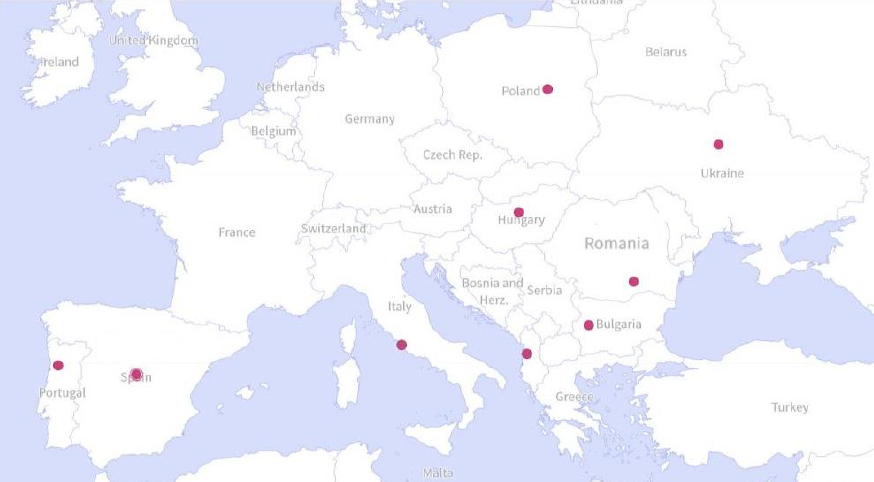
\includegraphics[width=12cm]{Imagem_1_Geral.png}
    \caption{Mapa com as cidades escolhidas.}
    \label{fig1}
\end{figure}

\newpage
\chapter{Questões}
\begin{itemize}
\item 1. Represente a situação escolhida por meio de um grafo.
\item 2. Indique, justificando, se o grafo é conexo.
No contexto do problema, interprete a sua resposta.
\item 3. Indique, justificando, se o grafo é euleriano.
No contexto do problema, interprete a sua resposta.
\item4. Indique, justificando, se o grafo é hamiltoniano.
No contexto do problema, interprete a sua resposta.
\item 5. Apresente a matriz de adjacência do grafo considerado na questão 1.
\item 6. Indique o fecho transitivo direto de um vértice à sua escolha.
No contexto do problema, apresente uma interpretação para o conjunto obtido.
\item 7. Indique o fecho transitivo inverso de um vértice à sua escolha.
No contexto do problema, apresente uma interpretação para o conjunto obtido.
\end{itemize}

\newpage
\subsection{Questão 1} %\subsubsection{objetivo A}
\textbf{Represente a situação escolhida por meio de um grafo.} 

\begin{figure}[h]
    \centering
    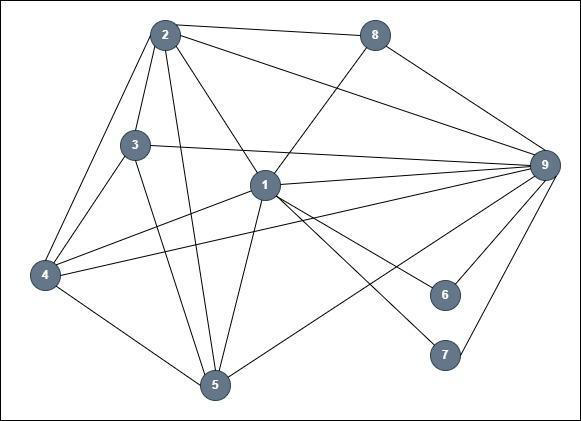
\includegraphics[width=12cm]{Imagem_2_Geral.png}
    \caption{Grafo G, Representação das ligações possíveis.}
    \label{fig2}
\end{figure}

\begin{center}
\begin{table}[h]
\centering
\begin{tabular}{r|r}
 1 & Madrid (Espanha); \\
 2 & Varsóvia Chopin (Polónia); \\ 
 3 & Porto (Portugal); \\
 4 & Kyiv Zhulyany (Ucrânia); \\
 5 & Budapeste (Hungria); \\
 6 & Bucareste H. Coanda (Roménia); \\
 7 & Sófia (Bulgária); \\
 8 & Tirana (Albânia); \\
 9 & Roma Fiumicino (Itália); 
 \end{tabular}
 \end{table}
 \end{center}
\textbf{V} = {1,2,3,4,5,6,7,8,9} \\
E = \\ (1,2),(1,4),(1,5),(1,6),(1,7),(1,8),(1,9),(2,1),(2,3),(2,4),(2,5),(2,8),(2,9),(3,2),\\(3,4),(3,5),(3,9),(4,1),(4,2),(4,3),(4,5),(4,9),(5,1),(5,2),(5,3),(5,4),(5,9),(6,1),\\(6,9),(7,1),(7,9),(8,1),(8,2),(8,9),(9,1),(9,2),(9,3),(9,4),(9,5),(9,6),(9,7),(9,8); 

\subsection{Questão 2} 
\textbf{Indique, justificando, se o grafo é conexo.} \cite{antero_2007}\\ 

O Grafo G só é conexo se existir uma cadeia que une quaisquer dois vértices, escolhidos ao acaso. Sendo assim, verifica-se que o Grafo G é conexo, pois, exemplificando, pode criar-se a cadeia \textbf{U = {3,2,1,7}}, partindo do vértice \textit{\textbf{Porto (v3)}}, de modo a chegar a \textit{\textbf{Sófia (v7)}}. Seguindo essa cadeia, inicia-se a partida através do \textbf{Porto}, com paragem em \textbf{Varsóvia}, seguido de \textbf{Madrid} e, por fim, com destino a \textbf{Sófia}.


\subsection{Questão 3}
\textbf{Indique, justificando, se o grafo é euleriano.} \\

Para um grafo ser euleriano, é necessário existir um ciclo euleriano. E, para isso, é necessária uma cadeia euleriana fechada, onde todas as arestas do grafo devem ser percorridas, sem serem repetidas. Deste modo, aplicam-se \underline{os dois teoremas} de \textbf{Euler} para perceber se há verificação deste ciclo no grafo acima exposto. \\
\\ Assim sendo: \\
\\
Pelo Teorema Euler (1): \\ 
\begin{itemize}
\item  Grafo G é conexo, verificado no ex.2.\\
\end{itemize}
É possível uma cadeia Euleriana?
deg(1)=7, deg(2)=6, deg(3)=4, deg(4)=5, deg(5)=5, deg(6)=2, deg(7)=2, deg(8)=3, deg(9)=8.\\
\\Não é possível uma cadeia Euleriana, pois possui mais de dois vértices de grau ímpar.\\
\\
Pelo, Teorema Euler (2):\\
\begin{itemize}
\item Grafo G é conexo, verificado no ex.2.\\
\end{itemize}
É possível um ciclo Euleriano?
\begin{itemize}
\item Não é possível um ciclo Euleriano, pois nem todos os vértices têm grau par.
\end{itemize}
\textbf{Conclusão}: \underline {Como verificado pelos teoremas, o grafo não é Euleriano.}

\subsection{Questão 4}
\textbf{Indique, justificando, se o grafo é hamiltoniano.} \\

Para o grafo G ser hamiltoniano, é necessário que seja possível formar um ciclo hamiltoniano que passe por todos os vértices de G, sem os repetir. Com ajuda de regras e teoremas, é possível comprovar se o grafo é ou não hamiltoniano. Pela \textit{\textbf{Regra 1}} constata-se que não é um grafo hamiltoniano, pois ambos os vértices, \textit{\textbf{v6}} e \textit{\textbf{v7}}, possuem arestas, cuja ligações torna incapaz a realização de um ciclo hamiltoniano, porque um dos vértices terá de ficar de fora para não se repetir. Caso contrário, repetir-se-ia o vértice \textit{\textbf{v1}} ou \textit{\textbf{v9}} para conseguir passar no \textit{\textbf{v6}} e \textit{\textbf{v7}}, o que implicaria a \textit{\textbf{Regra 3}}.

Pela \textit{\textbf{Regra 2}} deduz-se que não é um grafo hamiltoniano, pois pode sempre formar um ciclo antes de percorrer todos os vértices do grafo, conforme o Grafo G1.

\begin{figure}[h]
    \centering
    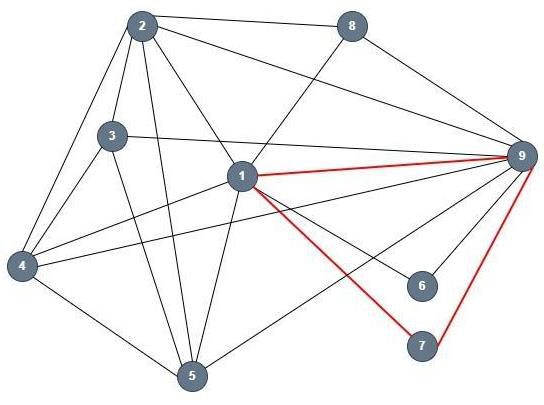
\includegraphics[width=12cm]{Imagem_3_Geral.png}
    \caption{Grafo G1, Ciclo já completo sem passar por todos os vértices.}
    \label{fig3}
\end{figure}

Pela \textit{\textbf{Regra 3}} confere-se que, também, que não é um grafo hamiltoniano, porque durante a construção do ciclo, se duas das arestas incidentes no vértice estão no mesmo, então todas as outras que incidem nesse vértice podem ser apagadas, ou seja, só se recorre a duas arestas por vértice. Logo os vértices não se podem repetir. \textbf{\textit{p.e.:}} para passar em \textit{\textbf{v6}} e \textit{\textbf{v7}} teríamos de repetir o \textit{\textbf{v1}} ou o \textbf{\textit{v9}}. Recorrendo ao \textit{Grafo G1}, observa-se que, removendo as arestas não pintadas dos vértices \textbf{\textit{v1}} e \textbf{\textit{v9}}, obtém-se com um ciclo isolado e com imensos vértices por visitar. Concomitantemente às regras supracitadas, os teoremas de \textbf{Dirac} e de \textbf{Ore} podem também informar da existência de ciclos hamiltonianos contidos no grafo.\\\\
Assim, segundo o \underline{\textbf{Teorema de Dirac}}:
\\\\
Seja \textit{G = (V, E)} um grafo simples, conexo, de ordem n >= 3, e se qualquer v tem deg(v) >= n / 2, então G tem um ciclo hamiltoniano.
\begin{itemize}
\item Grafo Simples, verifica-se pois não contém lacetes nem arestas múltiplas;
\item Conexo, verifica-se; \underline{\textit{verificado anteriormente}}.
\item 9 >= 3, verifica-se.
\end{itemize}
\\
\textbf{deg (1) =} 7 >= 9/2 \textbf{OK},\\
\textbf{deg (2) =} 6 >= 9/2 \textbf{OK},\\
\textbf{deg (8) =} 3 >= 9/2 \textbf{\textcolor{red}{NOK}}.
\\\\
\underline{\textbf{Por Dirac, nada podemos concluir}}.\\
\\
E pelo \underline{\textbf{Teorema de Ore}}:\\
\\
Seja \textit{G = (V, E}) um grafo simples, conexo, de ordem n >= 3, e se quaisquer vértices v1 ou v2 de G deg(v1) + deg(v2) >= n, então G tem um ciclo hamiltoniano.
\\
\begin{itemize}
\item Grafo Simples, verifica-se;
\item Conexo, verifica-se; \underline{\textit{verificado anteriormente.}}
\item 9 >= 3 verifica-se.
\end{itemize}
\textit{Vértices não adjacentes}:\\\\
deg (1) + deg (3) >= 9 \textbf{OK} \\
7 + 4 = 11;\\
deg (6) + deg (8) >= 9 \textcolor{red}{\textbf{NOK}} \\
2 + 3 = 5;\\
deg (4) + deg (8) >= 9 \textcolor{red}{\textbf{NOK}} \\
5 + 3 = 8;\\\\
\underline{\textbf{Por Ore, nada podemos concluir}}.\\\\
\textbf{Conclusão:} Pelas regras 1, 2 e 3, comprova-se que o \underline{\textit{\textbf{grafo não é hamiltoniano}}}. E, consoante os \textit{\textbf{Teoremas de Dirac}} e \textit{\textbf{Ore}}, nada podemos concluir.


\subsection{Questão 5}
Apresente a matriz de adjacência do grafo G, considerado na questão 1.\\
\citet{quaresma_2009}

\begin{table}[h]
    \centering
     \begin{tabular}{|c|c|c|c|c|c|c|c|c|c|}
        \hline
         & \textbf{V1} & \textbf{V2} & \textbf{V3} & \textbf{V4} & \textbf{V5} & \textbf{V6} & \textbf{V7} & \textbf{V8} & \textbf{V9} \\
        \hline 
        \textbf{V1} &  & \textbf{\textcolor{red}{1}} &  & \textbf{\textcolor{red}{1}} & \textbf{\textcolor{red}{1}} & \textbf{\textcolor{red}{1}} & \textbf{\textcolor{red}{1}} & \textbf{\textcolor{red}{1}} & \textbf{\textcolor{red}{1}} \\ 
        \hline
       \textbf{V2} & \textbf{\textcolor{red}{1}} &  & \textbf{\textcolor{red}{1}} & \textbf{\textcolor{red}{1}} & \textbf{\textcolor{red}{1}} &  &  & \textbf{\textcolor{red}{1}} & \textbf{\textcolor{red}{1}} \\
        \hline
       \textbf{V3} &  & \textbf{\textcolor{red}{1}} &  & \textbf{\textcolor{red}{1}} & \textbf{\textcolor{red}{1}} &  &  &  & \textbf{\textcolor{red}{1}} \\
        \hline
       \textbf{V4} & \textbf{\textcolor{red}{1}} & \textbf{\textcolor{red}{1}} & \textbf{\textcolor{red}{1}} &  & \textbf{\textcolor{red}{1}} &  &  &  & \textbf{\textcolor{red}{1}} \\
        \hline
        \textbf{V5} & \textbf{\textcolor{red}{1}} & \textbf{\textcolor{red}{1}} & \textbf{\textcolor{red}{1}} & \textbf{\textcolor{red}{1}} &  &  &  &  & \textbf{\textcolor{red}{1}} \\
        \hline
        \textbf{V6} & \textbf{\textcolor{red}{1}} &  &  &  &  &  &  &  & \textbf{\textcolor{red}{1}} \\
        \hline
        \textbf{V7} & \textbf{\textcolor{red}{1}} &  &  &  &  &  &  &  & \textbf{\textcolor{red}{1}}  \\
        \hline
        \textbf{V8} & \textbf{\textcolor{red}{1}} & \textbf{\textcolor{red}{1}} &  &  &  &  &  &  & \textbf{\textcolor{red}{1}} \\
        \hline
        \textbf{V9} & \textbf{\textcolor{red}{1}} & \textbf{\textcolor{red}{1}} & \textbf{\textcolor{red}{1}} & \textbf{\textcolor{red}{1}} & \textbf{\textcolor{red}{1}} & \textbf{\textcolor{red}{1}} & \textbf{\textcolor{red}{1}} & \textbf{\textcolor{red}{1}} & \\
        \hline
      \end{tabular}
    \caption{Matriz de Adjacência do Grafo G1.}
\end{table}

\subsection{Questão 6}
Indique o fecho transitivo direto de um vértice à sua escolha.\\
\cite{TeXnicCenter_2006}

\begin{table}[h]
    \centering
     \begin{tabular}{|c|c|c|c|c|c|c|c|c|c|c|}
        \hline
         & \textbf{V1} & \textbf{V2} & \textbf{V3} & \textbf{V4} & \textbf{V5} & \textbf{V6} & \textbf{V7} & \textbf{V8} & \textbf{V9} & \textit{\textbf{$\tau$}}3  \\
        \hline 
        \textbf{V1} &  & \textbf{\textcolor{red}{1}} &  & \textbf{\textcolor{red}{1}} & \textbf{\textcolor{red}{1}} & \textbf{\textcolor{red}{1}} & \textbf{\textcolor{red}{1}} & \textbf{\textcolor{red}{1}} & \textbf{\textcolor{red}{1}} & \textbf{\textcolor{blue}{2}}\\ 
        \hline
       \textbf{V2} & \textbf{\textcolor{red}{1}} &  & \textbf{\textcolor{red}{1}} & \textbf{\textcolor{red}{1}} & \textbf{\textcolor{red}{1}} &  &  & \textbf{\textcolor{red}{1}} & \textbf{\textcolor{red}{1}} & \textbf{\textcolor{blue}{1}} \\
        \hline
       \textbf{V3} &  & \textbf{\textcolor{red}{1}} &  & \textbf{\textcolor{red}{1}} & \textbf{\textcolor{red}{1}} &  &  &  & \textbf{\textcolor{red}{1}} & \textbf{\textcolor{blue}{0}}\\
        \hline
       \textbf{V4} & \textbf{\textcolor{red}{1}} & \textbf{\textcolor{red}{1}} & \textbf{\textcolor{red}{1}} &  & \textbf{\textcolor{red}{1}} &  &  &  & \textbf{\textcolor{red}{1}} & \textbf{\textcolor{blue}{1}}\\
        \hline
        \textbf{V5} & \textbf{\textcolor{red}{1}} & \textbf{\textcolor{red}{1}} & \textbf{\textcolor{red}{1}} & \textbf{\textcolor{red}{1}} &  &  &  &  & \textbf{\textcolor{red}{1}} & \textbf{\textcolor{blue}{1}}\\
        \hline
        \textbf{V6} & \textbf{\textcolor{red}{1}} &  &  &  &  &  &  &  & \textbf{\textcolor{red}{1}} & \textbf{\textcolor{blue}{2}}\\
        \hline
        \textbf{V7} & \textbf{\textcolor{red}{1}} &  &  &  &  &  &  &  & \textbf{\textcolor{red}{1}} & \textbf{\textcolor{blue}{2}}  \\
        \hline
        \textbf{V8} & \textbf{\textcolor{red}{1}} & \textbf{\textcolor{red}{1}} &  &  &  &  &  &  & \textbf{\textcolor{red}{1}} & \textbf{\textcolor{blue}{2}} \\
        \hline
        \textbf{V9} & \textbf{\textcolor{red}{1}} & \textbf{\textcolor{red}{1}} & \textbf{\textcolor{red}{1}} & \textbf{\textcolor{red}{1}} & \textbf{\textcolor{red}{1}} & \textbf{\textcolor{red}{1}} & \textbf{\textcolor{red}{1}} & \textbf{\textcolor{red}{1}} & & \textbf{\textcolor{blue}{1}} \\
        \hline
      \end{tabular}
    \caption{Tabela com fecho transitivo direto do Vértice 3, do grafo G.}
\end{table}
\newpage
\subsection{Questão 7}
Indique o fecho transitivo inverso de um vértice à sua escolha.\\
\cite{overleaf_1}

\begin{table}[h]
    \centering
     \begin{tabular}{|c|c|c|c|c|c|c|c|c|c|c|}
        \hline
         & \textbf{V1} & \textbf{V2} & \textbf{V3} & \textbf{V4} & \textbf{V5} & \textbf{V6} & \textbf{V7} & \textbf{V8} & \textbf{V9} & \textit{\textbf{$\tau$}}3 \\
        \hline 
        \textbf{V1} &  & \textbf{\textcolor{red}{1}} &  & \textbf{\textcolor{red}{1}} & \textbf{\textcolor{red}{1}} & \textbf{\textcolor{red}{1}} & \textbf{\textcolor{red}{1}} & \textbf{\textcolor{red}{1}} & \textbf{\textcolor{red}{1}} & \textbf{\textcolor{blue}{2}}\\ 
        \hline
       \textbf{V2} & \textbf{\textcolor{red}{1}} &  & \textbf{\textcolor{red}{1}} & \textbf{\textcolor{red}{1}} & \textbf{\textcolor{red}{1}} &  &  & \textbf{\textcolor{red}{1}} & \textbf{\textcolor{red}{1}} & \textbf{\textcolor{blue}{1}} \\
        \hline
       \textbf{V3} &  & \textbf{\textcolor{red}{1}} &  & \textbf{\textcolor{red}{1}} & \textbf{\textcolor{red}{1}} &  &  &  & \textbf{\textcolor{red}{1}} & \textbf{\textcolor{blue}{0}}\\
        \hline
       \textbf{V4} & \textbf{\textcolor{red}{1}} & \textbf{\textcolor{red}{1}} & \textbf{\textcolor{red}{1}} &  & \textbf{\textcolor{red}{1}} &  &  &  & \textbf{\textcolor{red}{1}} & \textbf{\textcolor{blue}{1}}\\
        \hline
        \textbf{V5} & \textbf{\textcolor{red}{1}} & \textbf{\textcolor{red}{1}} & \textbf{\textcolor{red}{1}} & \textbf{\textcolor{red}{1}} &  &  &  &  & \textbf{\textcolor{red}{1}} & \textbf{\textcolor{blue}{1}}\\
        \hline
        \textbf{V6} & \textbf{\textcolor{red}{1}} &  &  &  &  &  &  &  & \textbf{\textcolor{red}{1}} & \textbf{\textcolor{blue}{2}}\\
        \hline
        \textbf{V7} & \textbf{\textcolor{red}{1}} &  &  &  &  &  &  &  & \textbf{\textcolor{red}{1}} & \textbf{\textcolor{blue}{2}}  \\
        \hline
        \textbf{V8} & \textbf{\textcolor{red}{1}} & \textbf{\textcolor{red}{1}} &  &  &  &  &  &  & \textbf{\textcolor{red}{1}} & \textbf{\textcolor{blue}{2}} \\
        \hline
        \textbf{V9} & \textbf{\textcolor{red}{1}} & \textbf{\textcolor{red}{1}} & \textbf{\textcolor{red}{1}} & \textbf{\textcolor{red}{1}} & \textbf{\textcolor{red}{1}} & \textbf{\textcolor{red}{1}} & \textbf{\textcolor{red}{1}} & \textbf{\textcolor{red}{1}} & & \textbf{\textcolor{blue}{1}} \\
        \hline
        \textit{\textbf{$\tau$}}3$\wedge$(-1) & \textbf{\textcolor{blue}{2}} & \textbf{\textcolor{blue}{1}}
        & \textbf{\textcolor{blue}{0}} & \textbf{\textcolor{blue}{1}} & \textbf{\textcolor{blue}{1}} & \textbf{\textcolor{blue}{2}} & \textbf{\textcolor{blue}{2}} & \textbf{\textcolor{blue}{2}} & \textbf{\textcolor{blue}{1}} & \\
          \hline
         \end{tabular}         
    \caption{Tabela com fecho transitivo inverso do Vértice 3, do grafo G.}

\end{table}


\chapter{Conclusão}
\label{cap:conclusao} 
Neste trabalho abordámos a elaboração de um relatório utilizando a plataforma de Latex no âmbito da disciplina de \textbf {Laboratórios de Informática} usando assim o trabalho prático da disciplina de \textbf {Matemática Discreta} como conteúdo para a elaboração deste relatório. \\
Fomos capazes de concluir todos os objetivos propostos no TP04 da disciplina de Laboratórios de informática. \\
Este trabalho mostrou-se muito importante para compreemdermos melhor a elaboração de um relatório na plataforma de Latex, sendo que foi desafiante desenvolver o relatório sem recorrer à forma tradicional a que todos estamos habituados (Word). Ajudou-nos também a desenvolver competências de investigação, análise, organização e comunicação.

\end{document}
